\chapter{EVALUATION} \label{evaluation}
\begin{table}[tb]
\caption{Change in accuracy with embedding size.} % title of Table
\centering % used for centering table
\begin{tabular}{c c} % centered columns (4 columns)
\hline\hline %inserts double horizontal lines
Embedding Size(d) & Accuracy \\ [0.5ex] % inserts table
%heading
\hline % inserts single horizontal line
32 & 89.3 \\
64 & 93.8\\ % inserting body of the table
128 &  95.7\\[1ex] % [1ex] adds vertical space
\hline %inserts single line
\end{tabular}
\label{table:accuracyembedding} % is used to refer this table in the text
\end{table}

\begin{table}[tb]
\caption{Change in accuracy with number of filters.} % title of Table
\centering % used for centering table
\begin{tabular}{c c} % centered columns (4 columns)
\hline\hline %inserts double horizontal lines
Number of filters & Accuracy \\ [0.5ex] % inserts table
%heading
\hline % inserts single horizontal line
32 & 88.05 \\
64 & 95.7\\ % inserting body of the table
128 &  95.7\\[1ex] % [1ex] adds vertical space
\hline %inserts single line
\end{tabular}
\label{table:accuracyfilters} % is used to refer this table in the text
\end{table}



\section{Experiments}
Datasets used in the experiments are shown in Table~\ref{table:dataset}. For sentence classification, only blog articles and security reports were used.
From these articles, we further extracted two kinds of sentences, those with IOCs (IOC sentences) and those without but involving non-malicious IOC-like strings (non-IOC sentences). More specifically, the 5,000 IOC sentences and 2,500 non-IOC sentences were used in the experiments. These sentences are manually tagged by security experts to maintain the quality of data.

In the experiments, the parameters of our iGen (most of them related to CNN sub-module) system were set as follow:
\begin{itemize}
 \item[$\bullet$ ] \textit{Sequence length.} The length of our sentences before inputting them for classification. Remember that we padded all our sentences to have the same length of 70. We selected 70 as sequence length, since longest sentence in our dataset has 60 word length.
  \item[$\bullet$ ] \textit{Embedding Size.} The dimensionality of our word embeddings or word vectors is kept as 128. Word embedding dimensionality was chosen as 128 based on the experiments where we compared accuracy with dimensionality of word embeddings as shown in Table~\ref{table:accuracyembedding}. We did not increased the dimensionality beyond 128 as it has bad effect on the performance.   
  \item[$\bullet$ ] \textit{Filter Sizes.} Filter size is the number of words we want our convolutional filters to cover. We have used three type of filter 3, 4 and 5 that slide over 3, 4 and 5 words respectively. 
  \item[$\bullet$ ] \textit{Number of Filter.} It is number of filters per filter size. Based on the experiments shown in Table~\ref{table:accuracyfilters}, it is chosen as 64. Total $3*64$ filters are used with 64 filters each of size 3, 4, and 5.
  \item[$\bullet$ ] \textit{Dropout Keep Probability.} Dropout is the most popular method to regularize convolutional neural networks.A dropout layer stochastically disables a fraction of its neurons. This prevent neurons from co-adapting and forces them to learn individually useful features. The fraction of neurons we keep enabled is defined by the $dropout\char`_keep\char`_prob$ input to our network. We set this to something like 0.5 during training, and to 1 (disable dropout) during evaluation.
  
\end{itemize}

\section{Results}

\begin{figure*}[tb]
\centering
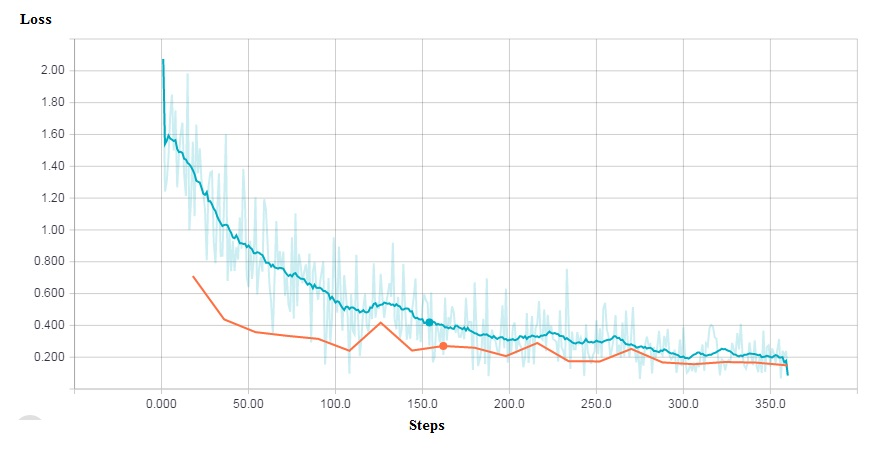
\includegraphics [width=\linewidth]{LossOverSteps.jpg}
\caption{Change in loss over steps (blue is training data, red is 10\% dev data).}
\label{fig:loss}
\end{figure*}

\begin{figure*}[tb]
\centering
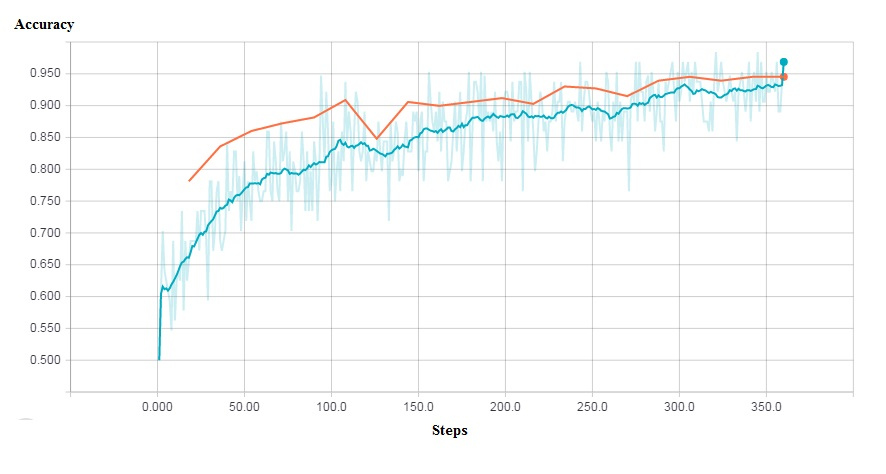
\includegraphics [width=\linewidth]{Accuracyoversteps.jpg}
\caption{Change in accuracy over steps (blue is training data, red is 10\% dev data).}
\label{fig:accuracy}
\end{figure*}

\subsection{Loss Function and Accuracy}


The loss is a measurement of the error our network makes, and our goal is to minimize it. The loss function for categorization problems is the cross-entropy loss.
$tf\cdot{nn}\cdot{softmax}\cdot{cross}\char`_entropy\char`_with\char`_logits$ is a function that calculates the cross-entropy loss for each class, given our scores and the correct input labels. We have then taken the mean of the losses. We could also use the sum, but that makes it harder to compare the loss across different batch sizes and train/dev data. Figure~\ref{fig:loss} shows the change cross-entropy loss over steps.

We also used an expression for the accuracy, which is a useful quantity to calculate the performance during training and testing. Change in accuracy over steps is shown in Figure~\ref{fig:accuracy}.

\subsection{Method Comparison}



We compared iGen with other state-of-the-art methods like Support Vector Machine (SVM)~\cite{cortes}, Naïve Bayes Classifier~\cite{nir}, and KNN (K-Nearest Neighbour)~\cite{liao1} classifier used for IOC sentence categorization. Three type of feature vector are used for each of the classifier described above. 10-fold cross validation technique is used to compare precision, recall and F-measure. Our comparative analysis is shown in Figure~\ref{table:methodcompare}.

iGen outperformed other methods by generating IOCs with a precision of 95\% and a recall of 99\%, while among other SVM with tfidf as feature vector performed well with a precision and recall of 90\%.

Similarly, another approach iACE~\cite{liao} proposed by Liao gave promising result in extracting IOC with high accuracy. But iACE used around 5,283 terms as features which were manually gathered from the dataset. This implies that it will work very accurately on one dataset but may fail on sentences where different terminologies were used while writing the article. In case of iGen, features were not selected manually but features were selected by CNN automatically. This property makes iGen more adaptive towards any kind of data. 
 

\begin{table}[tb]
\caption{Results of our iGen models against other methods. $\mathbf{SVM}$ (Support Vector Machine), $\mathbf{NB}$ (Naive Bayes), and $\mathbf{5-NN}$ (5-Nearest Neighbours) classifiers were compared with feature vectors as bag of words (BOW), term frequency (tf), and term frequency - inverse document frequency (tfidf).  } % title of Table
\centering % used for centering table
\begin{tabular}{c c c c} % centered columns (4 columns)
\hline\hline %inserts double horizontal lines
Methods & Precision & Recall & F-measure \\ [0.5ex] % inserts table
%heading
\hline % inserts single horizontal line
iGen & $\mathbf{95\%}$ & $\mathbf{99\%}$ & $\mathbf{97\%}$ \\
SVM (Bag of words) & 89\% & 88\% & 88\% \\ % inserting body of the table
SVM (tf) &  90\% & 89\% & 89\% \\
SVM (tfidf) &  90\% & 90\% & 90\% \\
Naive Bayes (Bag of words) & 81\% & 78\% & 79\% \\ % inserting body of the table
Naive Bayes (tf) &  83\% & 79\% & 81\% \\
Naive Bayes (tfidf) &  85\% & 83\% & 83\% \\
5-NN (Bag of words) & 80\% & 80\% & 80\% \\ % inserting body of the table
5-NN (tf) &  81\% & 81\% & 80\% \\
5-NN (tfidf) &  83\% & 82\% & 82\% \\[1ex] % [1ex] adds vertical space

\hline %inserts single line
\end{tabular}
\label{table:methodcompare} % is used to refer this table in the text
\end{table}